\documentclass[10pt,a4paper]{article}
\usepackage[margin=2.2cm]{geometry}
\usepackage{amsmath,amssymb,booktabs,graphicx,xcolor,hyperref,microtype,caption,enumitem}
\usepackage[numbers,sort&compress]{natbib}
\hypersetup{colorlinks=true,linkcolor=blue!50!black,citecolor=blue!50!black,urlcolor=blue!50!black}
\captionsetup{font=small,labelfont=bf}
\newcommand{\friedmanChi}{58.1}
\newcommand{\friedmanBlocks}{6}
\newcommand{\cdValue}{8.76}
\newcommand{\bestDetector}{Autoencoder}
\newcommand{\bestCleanAuc}{0.966}
\newcommand{\ensFprOne}{0.02}
\newcommand{\singleFprOne}{2.95}
\newcommand{\transferUU}{0.667}
\newcommand{\transferFprUU}{2}
\newcommand{\transferUC}{0.695}
\newcommand{\transferFprUC}{56}
\newcommand{\transferUCd}{0.610}
\newcommand{\transferFprUCd}{52}
\newcommand{\transferCC}{0.757}
\newcommand{\transferFprCC}{3}
\newcommand{\transferCU}{0.446}
\newcommand{\transferFprCU}{28}
\newcommand{\transferCUd}{0.550}
\newcommand{\transferFprCUd}{46}
\newcommand{\nmiNSL}{0.19}
\newcommand{\delThreeNSL}{51}
\newcommand{\delThreeRandNSL}{2}
\newcommand{\nDetectors}{15}
\newcommand{\nFlows}{22\,544}


\title{\textbf{Noctua: Unsupervised Network Intrusion Detection under\\Training Contamination, Temporal Drift and Dataset Shift}}
\author{Francisco Javier G\'omez Pulido\\\small Aapex \quad \texttt{github.com/fragompul/unsupervised-anomaly-network-intrusion}}
\date{October 2026}

\begin{document}
\maketitle

\begin{abstract}
Unsupervised detectors are attractive for intrusion detection because attack labels are scarce and attacks evolve, yet they are routinely evaluated on a clean training window, stationary traffic and a single network. We benchmark \nDetectors{} unsupervised detectors---tree, kernel, density, distance, reconstruction, deep one-class and self-supervised families, including a $\beta$-VAE, a RealNVP flow, a neural-transformation model and a masked tabular transformer---on NSL-KDD, UNSW-NB15 and CIC-IDS2017 under a protocol that removes those assumptions one at a time. Every detector is fit without labels and calibrated with split-conformal p-values, which turn any anomaly score into a false-positive guarantee that we then test to breaking. Three findings stand out. First, a few percent of hidden attacks in the training window degrades reconstruction and distance detectors by \meanDropFivePts{} ROC-AUC points on average at $\rho=5\%$ (up to \worstDropPts{} for \worstDropName{}). Second, \emph{Consensus-Trimmed Refit} (CTR), a label-free screen by three independent detectors, recovers \ctrGainFivePts{} points on average at $\rho=5\%$ and improves the plain detector in \ctrWinFraction{} dataset--detector pairs. Third, the conformal guarantee holds in-distribution but fails under drift and shift: the benign false-positive rate of a Monday-calibrated 1\% threshold is \driftBestFpr\% on the best day of CIC-IDS2017 (\driftBestDay) and \driftWorstFpr\% on the worst (\driftWorstDay), averaged over detectors, and a label-free population-stability index of the benign scores tracks this failure (Spearman $\rho=\psiSpearman$). Cross-dataset transfer between UNSW-NB15 and CIC-IDS2017 is poor (mean AUC \transferUC{} and \transferCU{}). We release the protocol, all raw scores, an interactive web laboratory, and code.
\end{abstract}

\section{Introduction}
Network intrusion detection is a one-class problem in disguise: normal behaviour is abundant, attacks are rare, labelled and non-stationary~\citep{sommer2010,arp2022}. Unsupervised and semi-supervised detectors therefore dominate the research literature, but they are usually evaluated under conditions that a deployment cannot guarantee: a curated attack-free training window, test traffic drawn from the training distribution, and a single dataset. When those conditions fail, headline AUCs say little about what an operator experiences, namely the \emph{false-alarm rate} at a threshold chosen in advance.

We study three questions. \textbf{(Q1) Contamination:} how much does a small fraction of undetected attacks in the training window hurt each detector family, and can it be repaired without labels? \textbf{(Q2) Drift:} how quickly does a threshold calibrated on one day stop meeting its false-positive budget, and is the breakdown visible without labels? \textbf{(Q3) Shift:} what survives when a detector trained on one network is deployed on another?

\paragraph{Contributions.} (i)~A reproducible protocol---label-free fitting, a held-out clean calibration slice, five experiments, bootstrap intervals and rank-based tests---over three public datasets that require no registration. (ii)~A conformal layer that gives every detector a finite-sample false-positive bound, a valid merge of heterogeneous detectors, and an empirical account of where the bound breaks. (iii)~Consensus-Trimmed Refit (CTR), a simple label-free defence against training contamination with ablations over trim level and screener committee. (iv)~A label-free drift alarm validated against calibration breakdown on real timestamps. (v)~Exact reconstruction attributions with a deletion-faithfulness test. (vi)~An interactive laboratory and all raw scores.

\section{Related work}
\paragraph{Anomaly detection benchmarks.} Surveys~\citep{chandola2009,pang2021} and ADBench~\citep{han2022} compare detectors on tabular data, usually under clean training and i.i.d.\ splits. Security-specific critiques~\citep{sommer2010,arp2022} stress that evaluation must respect time and deployment conditions; TESSERACT~\citep{pendlebury2019} does so for malware classification. We apply that discipline to unsupervised network detectors. Datasets used are NSL-KDD~\citep{tavallaee2009}, UNSW-NB15~\citep{moustafa2015} and CIC-IDS2017~\citep{sharafaldin2018}, whose labelling and flow-construction issues are documented~\citep{engelen2021}.

\paragraph{Detectors.} We include Isolation Forest~\citep{liu2008}, one-class SVM~\citep{scholkopf2001}, LOF~\citep{breunig2000}, ECOD~\citep{li2022}, COPOD~\citep{li2020}, HBOS~\citep{goldstein2012} through PyOD~\citep{zhao2019}, a Deep SVDD~\citep{ruff2018}, an autoencoder, a $\beta$-VAE~\citep{kingma2014,higgins2017}, a RealNVP flow~\citep{dinh2017}, NeuTraL AD~\citep{qiu2021} and a masked feature-reconstruction transformer in the spirit of FT-Transformer~\citep{gorishniy2021}.

\paragraph{Robustness and conformal methods.} Robust autoencoders~\citep{zhou2017} handle corrupted training data inside one model; CTR instead screens the data with a committee before any model is fit. Conformal prediction~\citep{vovk2005,angelopoulos2023} yields distribution-free guarantees; conformal p-values for outlier testing are analysed by~\citet{bates2023}, and p-values can be merged by averaging~\citep{vovk2020}. Drift detection on model outputs is studied by~\citet{rabanser2019}.

\section{Setting and protocol}
\paragraph{Data.} NSL-KDD (125,973 / 22,544 flows, 41 features), UNSW-NB15 (official 175,341 / 82,332 split, 34 features) and CIC-IDS2017 (2.83M flows, 78 features, timestamps), the latter subsampled class-aware (rare classes kept whole) and split temporally: Monday--Tuesday for training (Monday is attack-free), Wednesday--Friday for testing, so most test attack families are novel. For cross-dataset experiments UNSW-NB15 and CIC-IDS2017 are mapped to 18 physically aligned features. Identifiers (IPs, ports, flow id) are never features. All downloads are pinned by SHA-256 from public mirrors.

\paragraph{Contract and calibration.} A detector fits on unlabeled rows and returns a score, higher meaning more anomalous. Labels only score results. In every experiment 15\% of the training split's clean normal flows (at most 20k) are held out as a calibration set $\mathcal C$; conformal p-values are $p(s)=(1+|\{c\in\mathcal C: c\ge s\}|)/(|\mathcal C|+1)$, so that if calibration and test normals are exchangeable, $\Pr(p\le\alpha)\le\alpha$ for any detector~\citep{vovk2005}. The average $\min(1,2\bar p)$ of several such p-values is again valid~\citep{vovk2020}; for ranking we use the mean of $-\log_{10}p_k$. No hyperparameters are tuned on labels: every detector uses one fixed configuration across datasets.

\paragraph{Experiments.} \textbf{E1} main benchmark: all detectors, 3 datasets, \emph{clean} (normal-only) and \emph{natural} (training split as released) regimes, 5 seeds. \textbf{E2} contamination: attacks injected into a 30k-row normal base at $\rho\in\{0,1,2,5,10,20\}\%$. \textbf{E3} drift: fit and calibrate on Monday, evaluate Tuesday--Friday. \textbf{E4} shift: train on one dataset's harmonized clean normals, detect on the other, with source or per-domain standardization. Statistics follow Dem\v{s}ar~\citep{demsar2006}: Friedman tests, Nemenyi critical differences and Holm-corrected Wilcoxon tests over (dataset, regime, seed) blocks; because dataset splits are fixed, seeds are replicates over models and the tests are optimistic, which we say wherever they are used.

\section{Consensus-Trimmed Refit}
Attacks hidden in the training window are learned as normal by density, reconstruction and distance models. CTR removes them \emph{before} fitting: three structurally different cheap screeners (Isolation Forest, ECOD, PCA reconstruction) are fit on the training rows and score them; each score is converted to a percentile rank, the ranks are averaged, and the top $\tau$ fraction by consensus rank is dropped; the base detector is then fit on the remainder. The knob $\tau$ is an assumed upper bound on contamination. Agreement across independent inductive biases is a more specific contamination signal than any one detector's tail, which we test by ablation.

\section{Results}
\paragraph{E1: main benchmark.} Table~\ref{tab:main} gives ROC-AUC; Fig.~\ref{fig:cd} the critical-difference diagram (Friedman $\chi^2=\friedmanChi$ over \friedmanBlocks{} blocks, $\mathrm{CD}=\cdValue$); the best-ranked single detector is \bestDetector. The best clean-regime single-detector AUC is \bestCleanAuc. Averaged over single detectors in the clean regime the realized false-positive rate at a nominal $\alpha=1\%$ is \singleFprOne\%, whereas the conformal ensemble realizes \ensFprOne\%: merged p-values are conservative, and individual detectors over-alarm whenever test normals are not exchangeable with calibration normals (Fig.~\ref{fig:rel}).

\begin{table}[t]\centering\small
\begin{tabular}{lcc}
\toprule
 & \multicolumn{1}{c}{NSL-KDD-C} & \multicolumn{1}{c}{NSL-KDD-N} \\
\midrule
Autoencoder & \textbf{0.966} & 0.818 \\
kNN distance & 0.962 & 0.648 \\
$\beta$-VAE & 0.962 & 0.814 \\
Gaussian mixture & 0.959 & \textbf{0.931} \\
Deep SVDD & 0.957 & 0.734 \\
PCA reconstruction & 0.955 & 0.815 \\
ECOD & 0.952 & 0.903 \\
NeuTraL AD & 0.951 & 0.737 \\
Isolation Forest & 0.949 & 0.857 \\
COPOD & 0.949 & 0.897 \\
HBOS & 0.945 & 0.853 \\
RealNVP flow & 0.933 & 0.819 \\
Masked Tab-Transformer & 0.930 & 0.789 \\
One-Class SVM & 0.886 & 0.846 \\
Local Outlier Factor & 0.865 & 0.641 \\
\midrule
Ensemble (all) & 0.961 & 0.874 \\
Ensemble (diverse 5) & 0.960 & 0.816 \\
\bottomrule
\end{tabular}
\caption{ROC-AUC (mean over seeds). Columns: dataset and regime (C = clean, N = natural training). Bold: best single detector per column; ensembles listed last.}\label{tab:main}
\end{table}
\begin{figure}[t]\centering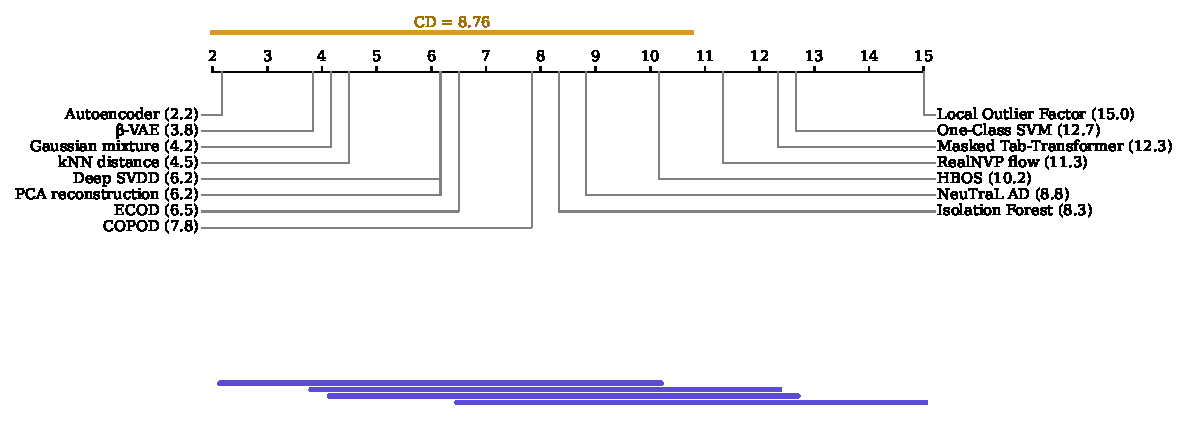
\includegraphics[width=.85\linewidth]{figures/cd.pdf}\caption{Critical-difference diagram (ROC-AUC). Methods joined by a bar are not significantly different (Nemenyi, $\alpha{=}0.05$).}\label{fig:cd}\end{figure}

\paragraph{E2: contamination.} Fig.~\ref{fig:contam} and Table~\ref{tab:contam} show the effect of hidden attacks. At $\rho=5\%$ the mean AUC drop is \meanDropFivePts{} points. CTR with a 10\% trim changes the AUC by \ctrGainFivePts{} points on average, and the ablation (Table~\ref{tab:abl}) compares trim levels, single screeners and an oracle trim equal to the true $\rho$.
\begin{figure}[t]\centering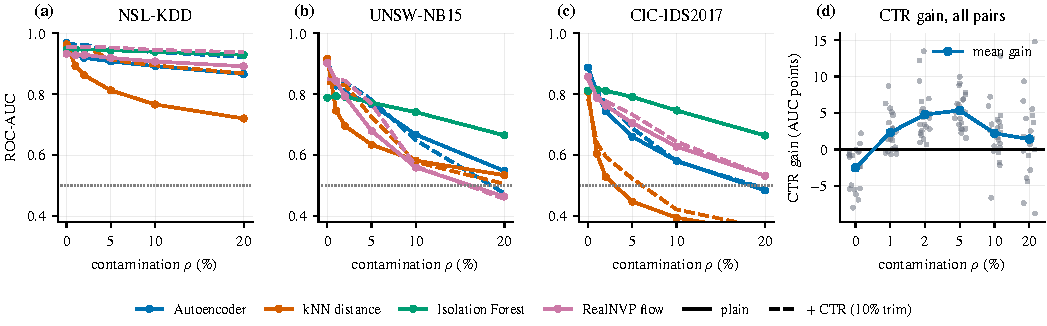
\includegraphics[width=\linewidth]{figures/contamination.pdf}\caption{ROC-AUC vs.\ training contamination. Solid: plain detector; dashed: behind CTR (trim 10\%).}\label{fig:contam}\end{figure}
\begin{table}[t]\centering\small\begin{tabular}{llrrrr}
\toprule
Dataset & Detector & $\rho{=}0$ & $\rho{=}5\%$ & + CTR & $\Delta$ \\
\midrule
NSL-KDD & Autoencoder & 0.968 & 0.907 & 0.944 & +0.037 \\
NSL-KDD & kNN distance & 0.962 & 0.812 & 0.912 & +0.100 \\
NSL-KDD & RealNVP flow & 0.933 & 0.918 & 0.953 & +0.034 \\
NSL-KDD & Gaussian mixture & 0.964 & 0.924 & 0.953 & +0.028 \\
\midrule
UNSW-NB15 & Autoencoder & 0.911 & 0.766 & 0.781 & +0.016 \\
UNSW-NB15 & kNN distance & 0.916 & 0.634 & 0.725 & +0.091 \\
UNSW-NB15 & RealNVP flow & 0.902 & 0.680 & 0.768 & +0.088 \\
UNSW-NB15 & Gaussian mixture & 0.901 & 0.651 & 0.719 & +0.068 \\
\midrule
CIC-IDS2017 & Autoencoder & 0.887 & 0.660 & 0.688 & +0.029 \\
CIC-IDS2017 & kNN distance & 0.807 & 0.447 & 0.523 & +0.075 \\
CIC-IDS2017 & RealNVP flow & 0.857 & 0.705 & 0.733 & +0.028 \\
CIC-IDS2017 & Gaussian mixture & 0.890 & 0.754 & 0.805 & +0.051 \\
\bottomrule
\end{tabular}\caption{Effect of 5\% contamination and CTR (mean over seeds).}\label{tab:contam}\end{table}
\begin{table}[t]\centering\small\begin{tabular}{lrrr}
\toprule
Training-set purification & NSL-KDD & UNSW-NB15 & CIC-IDS2017 \\
\midrule
No purification & 0.907 & 0.766 & 0.660 \\
\midrule
Committee, 5\% & 0.947 & 0.737 & 0.662 \\
Committee, 10\% (default) & 0.944 & 0.781 & 0.688 \\
Committee, 20\% & 0.960 & 0.817 & 0.697 \\
\midrule
IForest only, 10\% & 0.964 & 0.807 & 0.683 \\
ECOD only, 10\% & 0.961 & 0.827 & 0.684 \\
PCA only, 10\% & 0.933 & 0.678 & 0.646 \\
Oracle trim (5\%) & 0.947 & 0.737 & 0.662 \\
\bottomrule
\end{tabular}\caption{Ablation of CTR on the autoencoder at $\rho=5\%$ (ROC-AUC).}\label{tab:abl}\end{table}

\paragraph{E3: drift.} Fig.~\ref{fig:drift} (left) shows the realized benign false-positive rate by day for a Monday-calibrated 1\% threshold. Drift is \emph{not} monotone in time: averaged over single detectors the rate is \driftBestFpr\% on \driftBestDay{} and \driftWorstFpr\% on \driftWorstDay, because each day adds its own benign services. The population-stability index of benign scores, which needs no labels, correlates with the realized rate (Spearman $\rho=\psiSpearman$, Fig.~\ref{fig:drift} right). A PSI$\ge\alarmThr$ alarm flags the breakdown (FPR $\ge3\times$ nominal) with recall \alarmRecall\% and precision \alarmPrecision\%; the stricter PSI$\ge0.25$ threshold has precision \alarmHiPrecision\% but recall \alarmHiRecall\%, so the monitor is a conservative early warning rather than a complete one.
\begin{figure}[t]\centering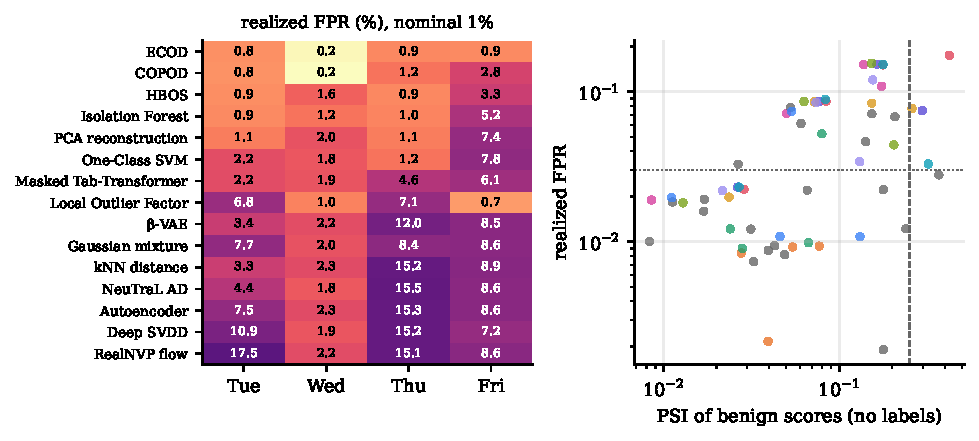
\includegraphics[width=\linewidth]{figures/drift.pdf}\caption{Left: realized FPR (\%) at nominal 1\% by day. Right: label-free PSI vs.\ realized FPR (dashed lines: PSI 0.25, FPR 3\%).}\label{fig:drift}\end{figure}
\begin{figure}[t]\centering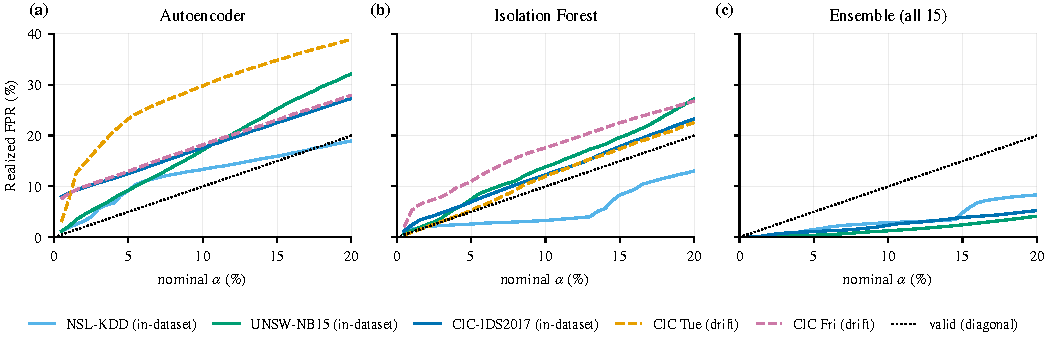
\includegraphics[width=\linewidth]{figures/reliability.pdf}\caption{Reliability diagrams: realized vs.\ nominal false-positive rate. On the diagonal the conformal guarantee holds; above it, it is broken.}\label{fig:rel}\end{figure}

\paragraph{E4: dataset shift.} Fig.~\ref{fig:transfer}: in-dataset mean AUC is \transferUU{} (UNSW) and \transferCC{} (CIC); transferred it is \transferUC{} (UNSW$\to$CIC) and \transferCU{} (CIC$\to$UNSW), with realized FPR at nominal 1\% of \transferFprUC\% and \transferFprCU\%. Per-domain standardization changes the transferred AUC to \transferUCd{} and \transferCUd{}.
\begin{figure}[t]\centering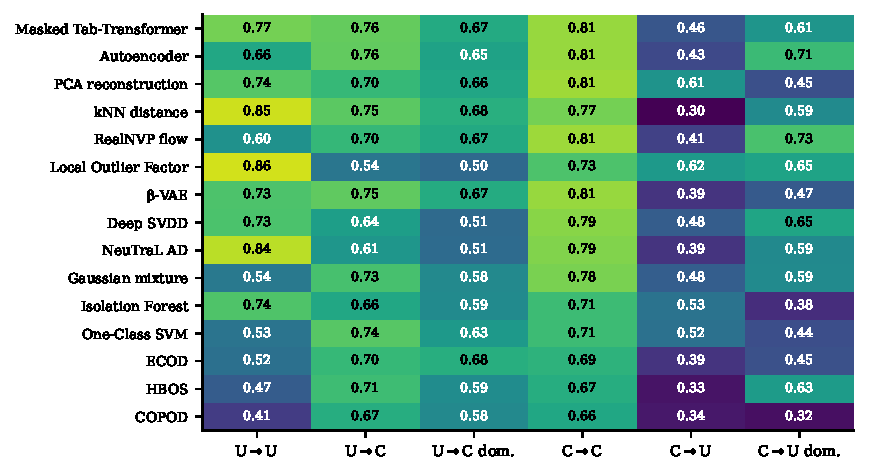
\includegraphics[width=.8\linewidth]{figures/transfer.pdf}\caption{ROC-AUC for in-dataset and cross-dataset evaluation on the 18-feature harmonized space (dom. = per-domain standardization).}\label{fig:transfer}\end{figure}

\paragraph{Explanations.} For the autoencoder, per-feature squared error is an exact additive decomposition of the score. Deleting the top-3 attributed features removes \delThreeNSL\%, \delThreeUNSW\% and \delThreeCIC\% of the score on NSL-KDD, UNSW-NB15 and CIC-IDS2017, against \delThreeRandNSL\%, \delThreeRandUNSW\% and \delThreeRandCIC\% for random features (Fig.~\ref{fig:explain}); k-means on attribution vectors of flagged flows recovers attack categories with NMI \nmiNSL{} / \nmiUNSW{} / \nmiCIC{}.
\begin{figure}[t]\centering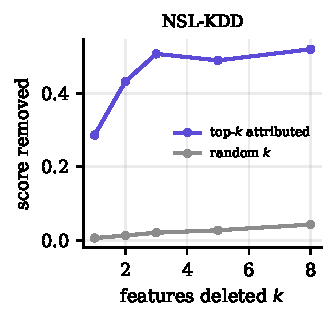
\includegraphics[width=.85\linewidth]{figures/explain.pdf}\caption{Deletion faithfulness of autoencoder attributions.}\label{fig:explain}\end{figure}

\section{Discussion and limitations}
Conformal calibration does what it promises when exchangeability holds, and it is precisely the diagnostic that reveals when it does not; this is more useful operationally than another AUC. Limitations (see the repository's \texttt{docs/limitations.md}): all datasets are lab-generated and have documented issues; fixed hyperparameters are fair across datasets but not optimal per dataset; seeds do not replicate datasets; CTR needs an assumed contamination bound; the harmonized transfer space is lossy; and we do not evaluate adaptive adversaries. Tabular foundation models such as TabPFN were examined for feasibility and excluded because per-feature conditional prediction is impractical on CPU at this scale.

\section{Conclusion}
Evaluating unsupervised intrusion detectors on a clean training window with a single threshold-free number hides exactly the failure modes that matter in deployment. A protocol that injects contamination, replays time and crosses networks, paired with conformal calibration and a label-free drift monitor, makes those failures measurable. Code, raw scores and an interactive laboratory accompany this paper.

\bibliographystyle{plainnat}
\bibliography{references}
\end{document}
